%
% 6.006 problem set 5 solutions template
%
\documentclass[12pt,twoside]{article}

\input{macros-sp20}
\newcommand{\theproblemsetnum}{5}

\title{6.006 Problem Set \theproblemsetnum}

\begin{document}

\handout{Problem Set \theproblemsetnum}

\setlength{\parindent}{0pt}
\medskip\hrulefill\medskip

{\bf Name:} Nicolas Iskandar

\medskip

{\bf Collaborators:} None

\medskip\hrulefill

\begin{problems}
\problem  % Problem 1

\begin{problemparts}
\problempart % Problem 1a
The matrix has edges $\{0,2\}, \{1,3\}, \{1,4\}, \{1,5\}, \{2,3\}, \{2,4\}, \{4,5\}$.
\begin{center}
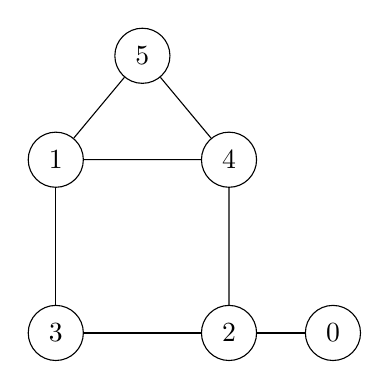
\begin{tikzpicture}[scale=1.1, every node/.style={circle, draw, minimum size=7mm, inner sep=0pt}]
  \node (n1) at (0,2)   {1};
  \node (n4) at (2,2)   {4};
  \node (n3) at (0,0)   {3};
  \node (n2) at (2,0)   {2};
  \node (n5) at (1,3.2) {5};
  \node (n0) at (3.2,0) {0};

  \draw (n1) -- (n3);
  \draw (n3) -- (n2);
  \draw (n2) -- (n4);
  \draw (n4) -- (n1);
  \draw (n5) -- (n1);
  \draw (n5) -- (n4);
  \draw (n0) -- (n2);
\end{tikzpicture}
\end{center}

\problempart % Problem 1b
{\color{dkgreen}}
\begin{lstlisting}
Adj = {
    'A': ['B'],
    'B': ['C', 'D'],
    'C': ['E', 'F'],
    'D': ['E', 'F'],
    'E': [],
    'F': ['D', 'E']
}
\end{lstlisting}

\problempart % Problem 1c
BFS visits vertices in order of distance from $A$, breaking ties alphabetically:
\[
[A, B, C, D, E, F].
\]
DFS plunges as deep as possible before backtracking, so after $A \to B \to C$, it goes $C \to E$, backtracks to visit $C \to F$, then $F \to D$ (since $D$ is still unvisited at that point):
\[
[A, B, C, E, F, D].
\]
The BFS tree has root $A$, child $B$, then $B$'s children $C, D$, then $C$'s children $E, F$. The DFS tree is the path $A \to B \to C \to E$ together with $C \to F \to D$.

\problempart % Problem 1d
The only cycle is between $D$ and $F$ (edges $(D,F)$ and $(F,D)$), so removing either edge makes the graph a DAG.

Removing $(D,F)$ leaves $(F,D)$, forcing $F$ before $D$; combined with the rest of the edges this pins down a unique order:
\[
(A, B, C, F, D, E).
\]

Removing $(F,D)$ leaves no edge between $C$ and $D$ at all, so they can appear in either order relative to each other, giving two valid orders:
\[
(A, B, C, D, F, E) \quad \text{and} \quad (A, B, D, C, F, E).
\]
\end{problemparts}

\problem  % Problem 2

Build an undirected graph $G$ on the $n$ plants and $n^2$ buildings, with an edge per wire. Since every building is powered by exactly one plant, each connected component of $G$ contains exactly one plant, and installing a backup generator at that plant benefits every other vertex in its component. So the best plant is the one in the largest connected component.

\textbf{Algorithm:} Run Full-BFS (or Full-DFS) on $G$ to compute the size of each component, then return the plant in the largest one.

\textbf{Running time:} $G$ has $O(n^2)$ vertices and $O(n^4)$ edges, so building $G$ and running Full-BFS both take $O(n^4)$ time.

\problem  % Problem 3

Build an undirected graph $G$ on the friends involved in at least one conflict, with an edge between each conflicting pair. Two peaceful parties exist if and only if $G$ is bipartite, since a valid party assignment is exactly a proper 2-coloring.

\textbf{Algorithm:} Run BFS on $G$ to build a spanning forest and record each vertex's distance from its component's source. Color vertices by the parity of that distance. Then check every edge: if any edge connects two same-colored vertices, no valid assignment exists (that edge, plus the even-length tree path between its endpoints, forms an odd cycle); otherwise the coloring works.

\textbf{Running time:} $G$ has $O(n)$ vertices and edges, so BFS and the edge check both take $O(n)$ time.

\problem  % Problem 4

Build a graph $G$ on the grid's $(n+1)^2$ intersections, connecting adjacent intersections unless doing so would cross between two squares owned by the same farmer. Paths in $G$ correspond exactly to legal (crop-preserving) routes.

To avoid running BFS separately from every euphris-adjacent intersection, add a supersource vertex $s$ connected to all of them. A single BFS from $s$ then finds the shortest path to the nearest tigrates-adjacent intersection, which is the desired trade route (dropping the artificial first edge from $s$).

\textbf{Running time:} $G$ has $O(n^2)$ vertices and edges, so building it and running one BFS both take $O(n^2)$ time.

\newpage
\problem  % Problem 5

Whether Liza can pass through a card-access door depends on which key cards she is currently carrying, so plain BFS on locations isn't enough. Since there are only 4 key card types plus a pizza flag, there are only $2^5 = 32$ possible states.

\textbf{Algorithm:} Duplicate each location into $32$ vertices, one per state $(\text{has pizza?}, \text{has SeeSail?}, \text{has TOPS?},\\ \text{has S3C?}, \text{has DPW?})$. Add an edge between two state-vertices whenever the corresponding door is traversable given the current cards, updating the state automatically if the destination holds a pizza or key card. Run BFS from the start state (at $e$, nothing held) to any state that has returned to $e$ while holding a pizza, and return the shortest such path.

\textbf{Running time:} The expanded graph is only a constant ($32\times$) factor larger than the original, so it has $O(|L|+|D|)$ vertices and edges, and one BFS takes $O(|L|+|D|)$ time.

\problem  % Problem 6

\begin{problemparts}
\problempart % Problem 6a
Each of the $s$ sliders can sit in any of the $n^2-b$ non-obstacle cells, and since sliders are otherwise indistinguishable, the number of ways to place them is
\[
\binom{n^2-b}{s} = \frac{1}{s!}\prod_{i=0}^{s-1}(n^2-b-i) = C(n,b,s).
\]
This overcounts reachable configurations, since obstacles and slider-blocking may make some placements physically unreachable by any sequence of tilts.

\problempart % Problem 6b
Each configuration has at most $r = 4$ successors, since there are only 4 tilt directions and each produces exactly one resulting configuration.

However, a configuration can have $\Omega(n^s)$ predecessors: take an obstacle-free board with $s \le n$ sliders each resting at the bottom of its own column. A `down' move reaches this exact configuration from \emph{any} starting arrangement with sliders in the same columns, regardless of their initial row, giving $n$ choices per slider, and $\Omega(n^s)$ possible predecessors overall.

\problempart % Problem 6c
Rather than building the full (possibly huge) configuration graph up front, run BFS starting from $B$, generating each configuration's successors lazily via the given \texttt{move} function only when that configuration is dequeued. Stop as soon as a configuration with a slider at the target square is found, and recover the move sequence via parent pointers.

Since BFS explores configurations in increasing order of moves taken, the first solved configuration found uses the minimum number of moves $k$.

\textbf{Running time:} If solvable in $k$ moves, BFS explores at most $\sum_{i=0}^k r^i = O(r^k)$ configurations before stopping, since each has at most $r=4$ successors. If unsolvable, BFS may need to explore all $C(n,b,s)$ reachable configurations. Each configuration costs $O(n^2)$ to expand, giving total time
\[
O\big(n^2 \cdot \min\{r^k,\ C(n,b,s)\}\big).
\]

\end{problemparts}

\end{problems}

\end{document}
